\documentclass[a4paper, 11pt]{article}

\usepackage{fullpage}
\usepackage[german]{babel}
%\usepackage[inline]{showlabels}
\usepackage{biblatex}
\usepackage{gnuplot-lua-tikz}
\usepackage{float}
\usepackage{amsmath}
\usepackage{graphicx}

\bibliography{E1.bib}

%kaliumion
\newcommand{\tVeinsKat}{$0,198$ }
\newcommand{\tVeinsAn}{$0,240$}
%hydroxyion
\newcommand{\tVzweiKat}{$0,802$ }
\newcommand{\tVzweiAn}{$0,760$ }

\newcommand{\VHzwei}{$1015,7\pm85,1\ µl$ }
\newcommand{\VOzwei}{$507,8\pm42,6\ µl$ }
\newcommand{\liteins}{$0,27$ }
\newcommand{\litzwei}{$0,73$ }
%Wanderungsgeschwindigkeit
\newcommand{\wanA}{$1,3\cdot 10^{-5}\ \frac{m}{s}$ }
\newcommand{\wanK}{$1,25\cdot 10^{-5}\ \frac{m}{s}$ }
%Überführungszahl teil 2
\newcommand{\UEK}{$5,28\cdot 10^{-8}$ }
\newcommand{\UEA}{$4,95\cdot 10^{-8}$ }
%Driftgeschwindigkeit
\newcommand{\DRiftK}{$1,35\cdot 10^{-8}\ \frac{m}{s}$ }
\newcommand{\DRiftA}{$1,44\cdot 10^{-8}\ \frac{m}{s}$ }

\title{Praktikum der Physikalischenchemie\\\large Ionenwanderung und Hittorfsche Überführungszahl}
\author{\\Samed Hür (huer@uni-bremen.de)\\Janosch Ehlers (jaeh@uni-bremen.de)\\\small Gruppe H\\ \\ \textbf{Betreuer:} Oliver Thüringer\\(thueringer@uni-bremen.de)}
\date{09.11.2022}

\begin{document}
\thispagestyle{empty}
\maketitle
\newpage

\tableofcontents
\thispagestyle{empty}
\newpage


Ziel der Versuche ist die Überführungszahlen der Ionen in einem Elektrolyten zu bestimmen, mit hilfe der Hittorf-Methode und der Methode der wanderenden Grenzfläche.
\section{Durchführung}
Als erstes wurden die drei Messzylinder gewogen. Anschließend wurden die Messzylinder mit 80\ ml $KOH$ gefüllt. Die gefüllten Messzylinder wurden gewogen, um den Volumenfehler des Messzylinders zu umgehen. Danach wurde das Dreikammer-Elektrolysegefäß mit der $KOH$- Lösung gefüllt. Anschließend wurden die Platin-Elektroden angebracht. Der Strom wurde angeschaltet. Während der Dauer von 90\ min wurde versucht die Stromstärke konstant auf 50\ mA zu halten. Währendessen wurde am Amfang jede Minute und ab 15\ min alle 5\ min die Stromstärke protokollliert. Zur Messung der Stromstärke wurde das Multimeter  Voltkraft M4660M verwendet, gemessen wurde auf der Einstellung 200\ mA. Außerdem wurden dreimal je 10\ ml $KOH$ zur kontrolle gegentitriert mit 0.1\ M $HCL$. Nach einer Messdauer von 90 Minuten wurde das Dreikammer-Elektrolysegefäß geleert. Anschließend wurde die $KOH$-Lösung ein letztes mal in den Messzylindern, die zum befüllen benutzt wurden, gewogen. Danach wurden zweimal 10\ ml  aus jeder Kammer titriert.
\begin{figure}[H]
\centering
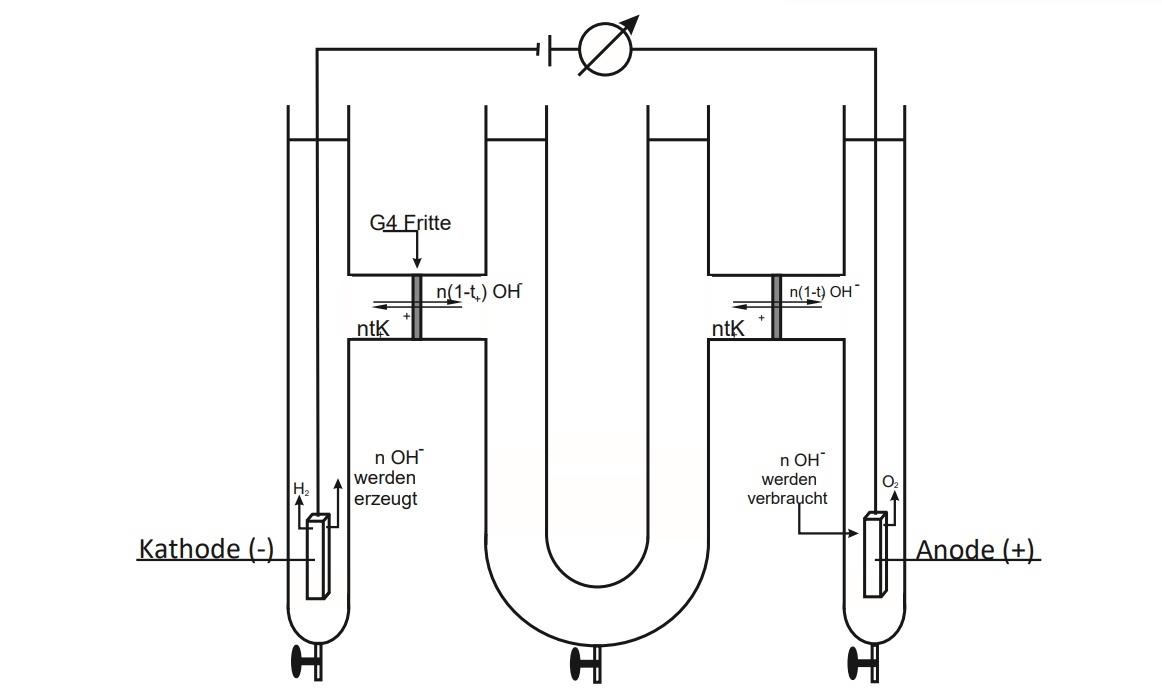
\includegraphics[scale=0.4]{Dreikammer.jpg}
\caption{Versuchsaufbau Teilversuch eins}
\end{figure}

Der Versuchteil 2 wurde nicht praktisch gemacht, Werte für den Versuchsteil 2 wurden uns bereitgestellt. 
Vor dem Versuch wurde Kontrolliert ob alle Geräte ausgeschaltet sind und auf 0 eingestellt sind, um Unfälle zu vermeiden da mit Gleichspannung gearbeitet wurde. Anschließend wurde der Pluspol des Spannungsgebers mit dem mA Eingang des Multimeters verbunden. Der COM Ausgang wurde mit der Anode des Elektrolysegefäßes Verbunden. Danach wurde die Kathode mit dem Minuspol des Spannungsgebers verbunden. Das untere Ende des U-Rohres ist über einem Stutzen mit Hahn mit einem Schlauch und einem Trichter verbunden. Die Vorbereitete Permanganat- Lösung wurde über einen Tropftrichter blasenfrei in den Schlauch gefüllt. Anschließend wurde der Hahn geöffnet um das gesamte Hahn-Volumen mit der Lösung zu fluten. Nach mehrmaligen ausspülen des U-Rohrs mit KNO$_{3}$-Lösung wurde das U-Rohr bis zur Hälfte der Schenkel befüllt. Danach werden die Elektroden eingehangen. Anschließend wurde der Hahn geöffnet um die KNO$_3$-Lösung mit der KMnO$_4$-Lösung zu unterschichten. Für eine scharfe Phasengrenzenausbildung werden die ersten cm innerhalb von einigen Minuten eingführt, dannach schneller. Die Elektrolyse wurde gestartet sobald die Elektroden ganz in der KNO$_3$-Lösung eingetaucht sind, und der Hahn geschlossen wurde. Die Elektrolyse dauert 20\ min bei 80\ v , dabei wurde alle 5\ min der Strom Protokoliert und die Position der Phasengrenzen an beiden Schenkel des U-Rohres markiert. 

\begin{figure}[H]
\centering
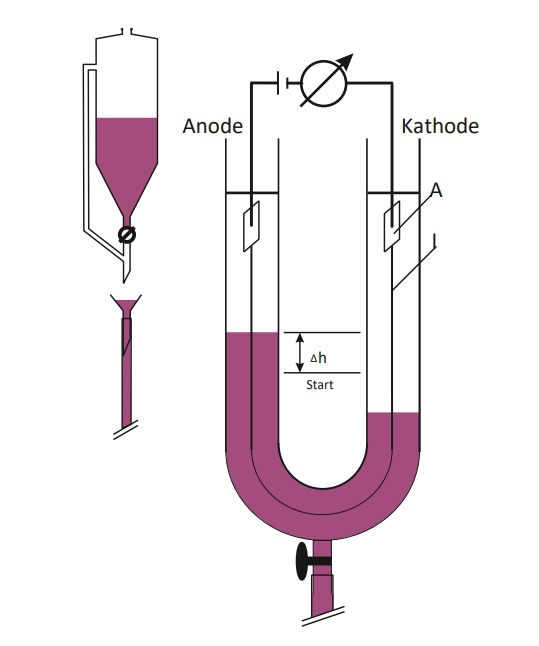
\includegraphics[scale=0.5]{Zweikammer.jpg}
\caption{Versuchsaufbau von Teilversuch zwei}
\end{figure}

\newpage
\section{Theoretischer Hintergrung}
Die Überführungszahl beschreibt den Bruchteil des gesamten Elektrischen Stromes, der von einer bestimmten Sorte Ionen transportiert wird. In einer Lösung mit nur zwei Ionenarten kann man die Überführungszahl mit $I_+/I$ berechnen. $I$ ist dabei der Gesamtstrom und $I_+$ der durch die Kationen transpotierte Strom.
Der Quotient der gesuchten Konzentrationsänderungen lässt sich über die Gleichung %1
$\frac{1}{t_-}-1$ überführen.
$$\frac{\Delta c_{Anodenraum}}{\Delta c_{Kathodenraum}} = \frac{t_+}{t_-} = \frac{1-t_-}{t_-} = \frac{1}{t_-}- 1$$
Bei der Elektrolyse wird nur das Hydroxion umgewandelt, während das Kaliumion unverändert in der Lösung verweilt. Daraus folgt: %2
$$\left|\Delta c_{Anodeenraum}\right| = \left|\Delta c_{Kathodenraum}\right|$$
Laut Definition ist die Ladung Q: %3
$$ Q= I\cdot t$$
Für die Überführungszahl gilt $t_+$: %4
$$t_+ = \frac{I_+}{I} = \frac{Q_+}{Q}$$
Das erste Faradaysche Gesetz bildet folgenden Zusammenhang: %5
$$Q_+ = \Delta n \cdot z \cdot F$$
Weiter folgt: %6
 $$t_+ = \frac{\Delta c_{Kathode}\cdot V_{Kathode}\cdot F \cdot  z_{Kation}}{Q} = - \frac{\Delta c_{Anode} \cdot V_{Anode} \cdot F \cdot z_{Kation}}{Q} $$
Für die Berechnung der Überführungszahl der Hydroxidionen gilt: %7
$$ t_+ + t_- = 1 $$
Alternativ erhalten wir die Überführungszahl aus einer Visuellen bestimmung.
In dem zweiten Versuchsaufbau wird eine Höhendifferenz ermittelt ($\Delta t$).Die Höhendifferenz ($\Delta t$) geteilt durch die Zeit ($t$) ergibt die Wandergeschwindigkeit: %8
$$V_{MnO4^-} = \frac{\Delta h}{t}$$
Mit dem Bezug auf das Elektrischesfeld wird die Ionenbeweglichkeit $U$ erhalten %9
$$ u_{MnO4^-} = \frac{u_{MnO4^-}}{\vec{E}} = \frac{u_{MnO4^-} \cdot l}{u}$$
Die molare Leitfähigkeit ist proportional zu der Ionenbeweglichkeit über: %10
$$\lambda_{MnO4^-} = zF\cdot u_{MnO4^-}$$
Für die Leidfähigkeit $\kappa$ der gesamten Lösung gilt: %11
$$\kappa = \frac{I}{U}\cdot \frac{l}{A}$$
Für die Überführungszahl $t$ gilt: %12
 $$ t_{MnO4^-} = \frac{\lambda_{MnO4^-} \cdot c_{MnO4^-}}{\kappa}$$

\newpage
\section{Chemikalienliste}
\subsection{Kaliumpermanganat}
\begin{itemize}
\item H272 Kann Brand verstärken; Oxidationsmittel.\\
\item H302 Gesundheitsschädlich bei Verschlucken.\\
\item H314 Verursacht schwere Verätzungen der Haut und schwere Augenschäden.\\
\item H361d Kann vermutlich das Kind im Mutterleib schädigen.\\
\item H373 Kann die Organe schädigen bei längerer oder wiederholter Exposition.
\item H410 Sehr giftig für Wasserorganismen mit langfristiger Wirkung.\\
\item P210 Von Hitze, heißen Oberflächen, Funken, offenen Flammen sowie anderen Zündquellenarten fernhalten. Nicht rauchen.\\
\item P220 Von Kleidung und anderen brennbaren Materialien fernhalten. \\
\item P280 Schutzhandschuhe / Schutzkleidung / Augenschutz / Gesichtsschutz tragen.\\
\item P301+P330+P331 Bei Verschlucken: Mund ausspülen. Kein Erbrechen herbeiführen. 
\item P303+P361+P353 Bei Berührung mit der Haut [oder dem Haar]: Alle kontaminierten Kleidungsstücke sofort ausziehen. Haut mit Wasser abwaschen [oder duschen]. 
\item P305+P351+P338 Bei Kontakt mit den Augen: Einige Minuten lang behutsam mit Wasser spülen. Eventuell vorhandene Kontaktlinsen nach Möglichkeit entfernen. Weiter spülen.
\item P310 Sofort Giftinformationszentrum, oder Arzt anrufen.\\
\end{itemize}

\subsection{Kaliumnitrat}
\begin{itemize}
\item H272 Kann Brand verstärken; Oxidationsmittel.\\
\item P210 Von Hitze, heißen Oberflächen, Funken, offenen Flammen sowie anderen Zündquellenarten fernhalten. Nicht rauchen.\\
\end{itemize}

\newpage
\begin{table}
\centering
\begin{tabular}{ccr}
$t\ [s]$& $I\ [mA]$		& $Q\ [C]$\\
\hline 
$0\pm 3$ 	& $51,25\pm0,256$	& 0\\
$60\pm 3$ 	& $50,03\pm0,25 $	& 3,0018\\
$120\pm 3$ 	& $50,03\pm0,25 $	& 6,0036\\
$180\pm 3$ 	& $50\pm0,25 	$	& 9\\
$240\pm 3$ 	& $49,99\pm0,25 $	& 11,9976\\
$300\pm 3$ 	& $50,01\pm0,25 $	& 15,003\\
$360\pm 3$ 	& $50\pm0,25 	$	& 18\\
$420\pm 3$ 	& $50\pm0,25 	$	& 21\\
$480\pm 3$ 	& $50\pm0,25 	$	& 24\\
$540\pm 3$ 	& $49,99\pm0,25 $	& 26,9946\\
$600\pm 3$ 	& $50,01\pm0,25 $	& 30,006\\
$660\pm 3$ 	& $49,99\pm0,25 $	& 32,9934\\
$720\pm 3$ 	& $50,01\pm0,25 $	& 36,0072\\
$780\pm 3$ 	& $49,98\pm0,25 $	& 38,9844\\
$840\pm 3$ 	& $49,99\pm0,25 $	& 41,9916\\
$900\pm 3$ 	& $49,98\pm0,25 $	& 44,982\\
$1200\pm 3$	& $50\pm0,25 	$	& 60\\
$1500\pm 3$ 	& $50\pm0,25 	$	& 75\\
$1800\pm 3$ 	& $50\pm0,25 	$	& 90\\
$2100\pm 3$ 	& $49,98\pm0,25 $	& 104,958\\
$2400\pm 3$ 	& $50,03\pm0,25 $	& 120,072\\
$2700\pm 3$ 	& $50,02\pm0,25 $	& 135,054\\
$3000\pm 3$ 	& $49,97\pm0,25 $	& 149,91\\
$3300\pm 3$ 	& $50\pm0,25 	$	& 165\\
$3600\pm 3$ 	& $49,99\pm0,25 $	& 179,964\\
$3900\pm 3$ 	& $49,99\pm0,25 $	& 194,961\\
$4200\pm 3$ 	& $50\pm0,25 	$	& 210\\
$4500\pm 3$ 	& $50\pm0,25 	$	& 225\\
$4800\pm 3$ 	& $49,98\pm0,25 $	& 239,904\\
$5100\pm 3$ 	& $49,99\pm0,25 $	& 254,949\\
$5400\pm 3$ 	& $50\pm0,25 	$	& 270\\
\end{tabular}
\caption{Rohdaten aus dem Versuchsteil eins}
\label{T1}
\end{table}
\newpage
\begin{figure}[H]
\centering
\begin{tikzpicture}[gnuplot]
%% generated with GNUPLOT 5.4p5 (Lua 5.4; terminal rev. Jun 2020, script rev. 115)
%% Fr 11 Nov 2022 16:47:57 CET
\path (0.000,0.000) rectangle (12.500,8.750);
\gpcolor{color=gp lt color border}
\gpsetlinetype{gp lt border}
\gpsetdashtype{gp dt solid}
\gpsetlinewidth{1.00}
\draw[gp path] (1.504,0.985)--(1.684,0.985);
\draw[gp path] (11.947,0.985)--(11.767,0.985);
\node[gp node right] at (1.320,0.985) {$49.6$};
\draw[gp path] (1.504,1.917)--(1.684,1.917);
\draw[gp path] (11.947,1.917)--(11.767,1.917);
\node[gp node right] at (1.320,1.917) {$49.7$};
\draw[gp path] (1.504,2.849)--(1.684,2.849);
\draw[gp path] (11.947,2.849)--(11.767,2.849);
\node[gp node right] at (1.320,2.849) {$49.8$};
\draw[gp path] (1.504,3.781)--(1.684,3.781);
\draw[gp path] (11.947,3.781)--(11.767,3.781);
\node[gp node right] at (1.320,3.781) {$49.9$};
\draw[gp path] (1.504,4.713)--(1.684,4.713);
\draw[gp path] (11.947,4.713)--(11.767,4.713);
\node[gp node right] at (1.320,4.713) {$50$};
\draw[gp path] (1.504,5.645)--(1.684,5.645);
\draw[gp path] (11.947,5.645)--(11.767,5.645);
\node[gp node right] at (1.320,5.645) {$50.1$};
\draw[gp path] (1.504,6.577)--(1.684,6.577);
\draw[gp path] (11.947,6.577)--(11.767,6.577);
\node[gp node right] at (1.320,6.577) {$50.2$};
\draw[gp path] (1.504,7.509)--(1.684,7.509);
\draw[gp path] (11.947,7.509)--(11.767,7.509);
\node[gp node right] at (1.320,7.509) {$50.3$};
\draw[gp path] (1.504,8.441)--(1.684,8.441);
\draw[gp path] (11.947,8.441)--(11.767,8.441);
\node[gp node right] at (1.320,8.441) {$50.4$};
\draw[gp path] (1.504,0.985)--(1.504,1.165);
\draw[gp path] (1.504,8.441)--(1.504,8.261);
\node[gp node center] at (1.504,0.677) {$0$};
\draw[gp path] (2.627,0.985)--(2.627,1.165);
\draw[gp path] (2.627,8.441)--(2.627,8.261);
\node[gp node center] at (2.627,0.677) {$10$};
\draw[gp path] (3.750,0.985)--(3.750,1.165);
\draw[gp path] (3.750,8.441)--(3.750,8.261);
\node[gp node center] at (3.750,0.677) {$20$};
\draw[gp path] (4.873,0.985)--(4.873,1.165);
\draw[gp path] (4.873,8.441)--(4.873,8.261);
\node[gp node center] at (4.873,0.677) {$30$};
\draw[gp path] (5.996,0.985)--(5.996,1.165);
\draw[gp path] (5.996,8.441)--(5.996,8.261);
\node[gp node center] at (5.996,0.677) {$40$};
\draw[gp path] (7.119,0.985)--(7.119,1.165);
\draw[gp path] (7.119,8.441)--(7.119,8.261);
\node[gp node center] at (7.119,0.677) {$50$};
\draw[gp path] (8.241,0.985)--(8.241,1.165);
\draw[gp path] (8.241,8.441)--(8.241,8.261);
\node[gp node center] at (8.241,0.677) {$60$};
\draw[gp path] (9.364,0.985)--(9.364,1.165);
\draw[gp path] (9.364,8.441)--(9.364,8.261);
\node[gp node center] at (9.364,0.677) {$70$};
\draw[gp path] (10.487,0.985)--(10.487,1.165);
\draw[gp path] (10.487,8.441)--(10.487,8.261);
\node[gp node center] at (10.487,0.677) {$80$};
\draw[gp path] (11.610,0.985)--(11.610,1.165);
\draw[gp path] (11.610,8.441)--(11.610,8.261);
\node[gp node center] at (11.610,0.677) {$90$};
\draw[gp path] (1.504,8.441)--(1.504,0.985)--(11.947,0.985)--(11.947,8.441)--cycle;
\node[gp node center,rotate=-270] at (0.292,4.713) {Stromstärke [mA]};
\node[gp node center] at (6.725,0.215) {Zeit [s]};
\gpcolor{rgb color={0.580,0.000,0.827}}
\draw[gp path] (1.616,2.663)--(1.616,7.323);
\draw[gp path] (1.526,2.663)--(1.706,2.663);
\draw[gp path] (1.526,7.323)--(1.706,7.323);
\draw[gp path] (1.729,2.663)--(1.729,7.323);
\draw[gp path] (1.639,2.663)--(1.819,2.663);
\draw[gp path] (1.639,7.323)--(1.819,7.323);
\draw[gp path] (1.841,2.383)--(1.841,7.043);
\draw[gp path] (1.751,2.383)--(1.931,2.383);
\draw[gp path] (1.751,7.043)--(1.931,7.043);
\draw[gp path] (1.953,2.290)--(1.953,6.950);
\draw[gp path] (1.863,2.290)--(2.043,2.290);
\draw[gp path] (1.863,6.950)--(2.043,6.950);
\draw[gp path] (2.065,2.476)--(2.065,7.136);
\draw[gp path] (1.975,2.476)--(2.155,2.476);
\draw[gp path] (1.975,7.136)--(2.155,7.136);
\draw[gp path] (2.178,2.383)--(2.178,7.043);
\draw[gp path] (2.088,2.383)--(2.268,2.383);
\draw[gp path] (2.088,7.043)--(2.268,7.043);
\draw[gp path] (2.290,2.383)--(2.290,7.043);
\draw[gp path] (2.200,2.383)--(2.380,2.383);
\draw[gp path] (2.200,7.043)--(2.380,7.043);
\draw[gp path] (2.402,2.383)--(2.402,7.043);
\draw[gp path] (2.312,2.383)--(2.492,2.383);
\draw[gp path] (2.312,7.043)--(2.492,7.043);
\draw[gp path] (2.515,2.290)--(2.515,6.950);
\draw[gp path] (2.425,2.290)--(2.605,2.290);
\draw[gp path] (2.425,6.950)--(2.605,6.950);
\draw[gp path] (2.627,2.476)--(2.627,7.136);
\draw[gp path] (2.537,2.476)--(2.717,2.476);
\draw[gp path] (2.537,7.136)--(2.717,7.136);
\draw[gp path] (2.739,2.290)--(2.739,6.950);
\draw[gp path] (2.649,2.290)--(2.829,2.290);
\draw[gp path] (2.649,6.950)--(2.829,6.950);
\draw[gp path] (2.851,2.476)--(2.851,7.136);
\draw[gp path] (2.761,2.476)--(2.941,2.476);
\draw[gp path] (2.761,7.136)--(2.941,7.136);
\draw[gp path] (2.964,2.197)--(2.964,6.857);
\draw[gp path] (2.874,2.197)--(3.054,2.197);
\draw[gp path] (2.874,6.857)--(3.054,6.857);
\draw[gp path] (3.076,2.290)--(3.076,6.950);
\draw[gp path] (2.986,2.290)--(3.166,2.290);
\draw[gp path] (2.986,6.950)--(3.166,6.950);
\draw[gp path] (3.188,2.197)--(3.188,6.857);
\draw[gp path] (3.098,2.197)--(3.278,2.197);
\draw[gp path] (3.098,6.857)--(3.278,6.857);
\draw[gp path] (3.750,2.383)--(3.750,7.043);
\draw[gp path] (3.660,2.383)--(3.840,2.383);
\draw[gp path] (3.660,7.043)--(3.840,7.043);
\draw[gp path] (4.311,2.383)--(4.311,7.043);
\draw[gp path] (4.221,2.383)--(4.401,2.383);
\draw[gp path] (4.221,7.043)--(4.401,7.043);
\draw[gp path] (4.873,2.383)--(4.873,7.043);
\draw[gp path] (4.783,2.383)--(4.963,2.383);
\draw[gp path] (4.783,7.043)--(4.963,7.043);
\draw[gp path] (5.434,2.197)--(5.434,6.857);
\draw[gp path] (5.344,2.197)--(5.524,2.197);
\draw[gp path] (5.344,6.857)--(5.524,6.857);
\draw[gp path] (5.996,2.663)--(5.996,7.323);
\draw[gp path] (5.906,2.663)--(6.086,2.663);
\draw[gp path] (5.906,7.323)--(6.086,7.323);
\draw[gp path] (6.557,2.569)--(6.557,7.229);
\draw[gp path] (6.467,2.569)--(6.647,2.569);
\draw[gp path] (6.467,7.229)--(6.647,7.229);
\draw[gp path] (7.119,2.103)--(7.119,6.763);
\draw[gp path] (7.029,2.103)--(7.209,2.103);
\draw[gp path] (7.029,6.763)--(7.209,6.763);
\draw[gp path] (7.680,2.383)--(7.680,7.043);
\draw[gp path] (7.590,2.383)--(7.770,2.383);
\draw[gp path] (7.590,7.043)--(7.770,7.043);
\draw[gp path] (8.241,2.290)--(8.241,6.950);
\draw[gp path] (8.151,2.290)--(8.331,2.290);
\draw[gp path] (8.151,6.950)--(8.331,6.950);
\draw[gp path] (8.803,2.290)--(8.803,6.950);
\draw[gp path] (8.713,2.290)--(8.893,2.290);
\draw[gp path] (8.713,6.950)--(8.893,6.950);
\draw[gp path] (9.364,2.383)--(9.364,7.043);
\draw[gp path] (9.274,2.383)--(9.454,2.383);
\draw[gp path] (9.274,7.043)--(9.454,7.043);
\draw[gp path] (9.926,2.383)--(9.926,7.043);
\draw[gp path] (9.836,2.383)--(10.016,2.383);
\draw[gp path] (9.836,7.043)--(10.016,7.043);
\draw[gp path] (10.487,2.197)--(10.487,6.857);
\draw[gp path] (10.397,2.197)--(10.577,2.197);
\draw[gp path] (10.397,6.857)--(10.577,6.857);
\draw[gp path] (11.049,2.290)--(11.049,6.950);
\draw[gp path] (10.959,2.290)--(11.139,2.290);
\draw[gp path] (10.959,6.950)--(11.139,6.950);
\draw[gp path] (11.610,2.383)--(11.610,7.043);
\draw[gp path] (11.520,2.383)--(11.700,2.383);
\draw[gp path] (11.520,7.043)--(11.700,7.043);
\gpcolor{color=gpbgfillcolor}
\gpsetpointsize{4.00}
\gp3point{gp mark 7}{}{(1.616,4.993)}
\gpcolor{rgb color={0.580,0.000,0.827}}
\gp3point{gp mark 1}{}{(1.616,4.993)}
\gpcolor{color=gpbgfillcolor}
\gp3point{gp mark 7}{}{(1.729,4.993)}
\gpcolor{rgb color={0.580,0.000,0.827}}
\gp3point{gp mark 1}{}{(1.729,4.993)}
\gpcolor{color=gpbgfillcolor}
\gp3point{gp mark 7}{}{(1.841,4.713)}
\gpcolor{rgb color={0.580,0.000,0.827}}
\gp3point{gp mark 1}{}{(1.841,4.713)}
\gpcolor{color=gpbgfillcolor}
\gp3point{gp mark 7}{}{(1.953,4.620)}
\gpcolor{rgb color={0.580,0.000,0.827}}
\gp3point{gp mark 1}{}{(1.953,4.620)}
\gpcolor{color=gpbgfillcolor}
\gp3point{gp mark 7}{}{(2.065,4.806)}
\gpcolor{rgb color={0.580,0.000,0.827}}
\gp3point{gp mark 1}{}{(2.065,4.806)}
\gpcolor{color=gpbgfillcolor}
\gp3point{gp mark 7}{}{(2.178,4.713)}
\gpcolor{rgb color={0.580,0.000,0.827}}
\gp3point{gp mark 1}{}{(2.178,4.713)}
\gpcolor{color=gpbgfillcolor}
\gp3point{gp mark 7}{}{(2.290,4.713)}
\gpcolor{rgb color={0.580,0.000,0.827}}
\gp3point{gp mark 1}{}{(2.290,4.713)}
\gpcolor{color=gpbgfillcolor}
\gp3point{gp mark 7}{}{(2.402,4.713)}
\gpcolor{rgb color={0.580,0.000,0.827}}
\gp3point{gp mark 1}{}{(2.402,4.713)}
\gpcolor{color=gpbgfillcolor}
\gp3point{gp mark 7}{}{(2.515,4.620)}
\gpcolor{rgb color={0.580,0.000,0.827}}
\gp3point{gp mark 1}{}{(2.515,4.620)}
\gpcolor{color=gpbgfillcolor}
\gp3point{gp mark 7}{}{(2.627,4.806)}
\gpcolor{rgb color={0.580,0.000,0.827}}
\gp3point{gp mark 1}{}{(2.627,4.806)}
\gpcolor{color=gpbgfillcolor}
\gp3point{gp mark 7}{}{(2.739,4.620)}
\gpcolor{rgb color={0.580,0.000,0.827}}
\gp3point{gp mark 1}{}{(2.739,4.620)}
\gpcolor{color=gpbgfillcolor}
\gp3point{gp mark 7}{}{(2.851,4.806)}
\gpcolor{rgb color={0.580,0.000,0.827}}
\gp3point{gp mark 1}{}{(2.851,4.806)}
\gpcolor{color=gpbgfillcolor}
\gp3point{gp mark 7}{}{(2.964,4.527)}
\gpcolor{rgb color={0.580,0.000,0.827}}
\gp3point{gp mark 1}{}{(2.964,4.527)}
\gpcolor{color=gpbgfillcolor}
\gp3point{gp mark 7}{}{(3.076,4.620)}
\gpcolor{rgb color={0.580,0.000,0.827}}
\gp3point{gp mark 1}{}{(3.076,4.620)}
\gpcolor{color=gpbgfillcolor}
\gp3point{gp mark 7}{}{(3.188,4.527)}
\gpcolor{rgb color={0.580,0.000,0.827}}
\gp3point{gp mark 1}{}{(3.188,4.527)}
\gpcolor{color=gpbgfillcolor}
\gp3point{gp mark 7}{}{(3.750,4.713)}
\gpcolor{rgb color={0.580,0.000,0.827}}
\gp3point{gp mark 1}{}{(3.750,4.713)}
\gpcolor{color=gpbgfillcolor}
\gp3point{gp mark 7}{}{(4.311,4.713)}
\gpcolor{rgb color={0.580,0.000,0.827}}
\gp3point{gp mark 1}{}{(4.311,4.713)}
\gpcolor{color=gpbgfillcolor}
\gp3point{gp mark 7}{}{(4.873,4.713)}
\gpcolor{rgb color={0.580,0.000,0.827}}
\gp3point{gp mark 1}{}{(4.873,4.713)}
\gpcolor{color=gpbgfillcolor}
\gp3point{gp mark 7}{}{(5.434,4.527)}
\gpcolor{rgb color={0.580,0.000,0.827}}
\gp3point{gp mark 1}{}{(5.434,4.527)}
\gpcolor{color=gpbgfillcolor}
\gp3point{gp mark 7}{}{(5.996,4.993)}
\gpcolor{rgb color={0.580,0.000,0.827}}
\gp3point{gp mark 1}{}{(5.996,4.993)}
\gpcolor{color=gpbgfillcolor}
\gp3point{gp mark 7}{}{(6.557,4.899)}
\gpcolor{rgb color={0.580,0.000,0.827}}
\gp3point{gp mark 1}{}{(6.557,4.899)}
\gpcolor{color=gpbgfillcolor}
\gp3point{gp mark 7}{}{(7.119,4.433)}
\gpcolor{rgb color={0.580,0.000,0.827}}
\gp3point{gp mark 1}{}{(7.119,4.433)}
\gpcolor{color=gpbgfillcolor}
\gp3point{gp mark 7}{}{(7.680,4.713)}
\gpcolor{rgb color={0.580,0.000,0.827}}
\gp3point{gp mark 1}{}{(7.680,4.713)}
\gpcolor{color=gpbgfillcolor}
\gp3point{gp mark 7}{}{(8.241,4.620)}
\gpcolor{rgb color={0.580,0.000,0.827}}
\gp3point{gp mark 1}{}{(8.241,4.620)}
\gpcolor{color=gpbgfillcolor}
\gp3point{gp mark 7}{}{(8.803,4.620)}
\gpcolor{rgb color={0.580,0.000,0.827}}
\gp3point{gp mark 1}{}{(8.803,4.620)}
\gpcolor{color=gpbgfillcolor}
\gp3point{gp mark 7}{}{(9.364,4.713)}
\gpcolor{rgb color={0.580,0.000,0.827}}
\gp3point{gp mark 1}{}{(9.364,4.713)}
\gpcolor{color=gpbgfillcolor}
\gp3point{gp mark 7}{}{(9.926,4.713)}
\gpcolor{rgb color={0.580,0.000,0.827}}
\gp3point{gp mark 1}{}{(9.926,4.713)}
\gpcolor{color=gpbgfillcolor}
\gp3point{gp mark 7}{}{(10.487,4.527)}
\gpcolor{rgb color={0.580,0.000,0.827}}
\gp3point{gp mark 1}{}{(10.487,4.527)}
\gpcolor{color=gpbgfillcolor}
\gp3point{gp mark 7}{}{(11.049,4.620)}
\gpcolor{rgb color={0.580,0.000,0.827}}
\gp3point{gp mark 1}{}{(11.049,4.620)}
\gpcolor{color=gpbgfillcolor}
\gp3point{gp mark 7}{}{(11.610,4.713)}
\gpcolor{rgb color={0.580,0.000,0.827}}
\gp3point{gp mark 1}{}{(11.610,4.713)}
\gpcolor{color=gp lt color border}
\draw[gp path] (1.504,8.441)--(1.504,0.985)--(11.947,0.985)--(11.947,8.441)--cycle;
%% coordinates of the plot area
\gpdefrectangularnode{gp plot 1}{\pgfpoint{1.504cm}{0.985cm}}{\pgfpoint{11.947cm}{8.441cm}}
\end{tikzpicture}
%% gnuplot variables

\caption{Graphische Darstellung der Rohdaten aus Tabelle \ref{T1}}
\label{abb1}
\end{figure}

\section{Auswertung}
\subsection{Versuchteil eins}
Mit der Hittorf-Methode konnte die Überführungszahl einer 0,1 molaren KOH-Lösung ermittelt werden. 
Die Überführungszahl des Kaliumions beträgt im Kathodenraum \tVeinsKat und im Anodenraum \tVeinsAn. 
Die Überführungszahl des Hydroxidions beträgt im Kathodenraum \tVzweiKat und im Anodenraum \tVzweiAn. 
Die Überführungszahlen stimmen innerhalb ihrer Fehlergrenzen mit den Literaturwerten\cite{Lit} über ein, mit \liteins für die Kaliumionen und \litzwei für die Hydroxidionen bei Raumtemperatur.\\
Einige Fehler für diesen Versuch wurden geschätzt.
$\Delta t$ wurde auf $3\ s$ und die Dichte von Wasser wurde auf $\Delta\rho=0,0001\ \frac{g}{mol}$ geschätzt, während der Strom Fehler aus der Betriebsanweisung\cite{Multimeter} des Messgerätes hervorgeht. $\Delta I = 0,5\% \wedge 3\ digits$.

\begin{table}[H]
\centering
\begin{tabular}{lccc}
		& Kat-		& Mittel-	& An-\\
\hline
Leergewicht 	& 108,44 	& 117,93 	& 108,21\\
Vollgewicht A 	& 187,23 	& 196,9 	& 187,06\\
Vollgewicht E 	& 179,34 	& 197,78 	& 191,57\\
Volumen A 	& 78,93 	& 79,11 	& 78,99\\
Volumen E 	& 71,03 	& 79,99 	& 83,51\\
Titration E1 	& 7,85 		& 8,8 		& 9,85\\
Titration E2 	& 7,75 		& 8,95 		& 9,65\\
$c(KOH)_1$	& 0,0785 	& 0,088 	& 0,0985\\
$c(KOH)_2$	& 0,0775 	& 0,0895 	& 0,0965\\
$\bar{\Delta c}(KOH)$ & 0,015 	& 0,00075 	& 0,0085\\
\end{tabular}
\caption{Relevante Volumina und Gewichte}
\label{T2}
\end{table}



Anschließend wurde die Überführte Ladung $Q$ nach $Q=t\cdot I$ berechnet. Der Fehler der Ladung ($\Delta Q$) entspricht Gleichung \ref{q_aus_tI}.

\begin{equation}
Q = t \cdot I
\label{q_aus_tI}
\end{equation}
Weiter Berechnet sich der Fehler der Ladung nach Gleichung \ref{dQ}.

\begin{equation}
\Delta Q=\sqrt{\left(\Delta t\cdot I\right)^2 + \left(\Delta I\cdot t\right)^2}
\label{dQ}
\end{equation}

\begin{equation}
 269.9928\ C = 269.9928\ A\cdot s = 5400\ s \cdot 49.998\ mA \cdot 0.001\ \frac{A}{mA}
\label{BSPq}
\end{equation}

\begin{equation}
\Delta Q=\sqrt{\left(3\ s\cdot 50,00\ mA\right)^2 + \left(0,00025\ mA\cdot 5400\ s\right)^2}= 1,36\ C
\label{BSPdq}
\end{equation}
Beispielhaft ist in Gleichung \ref{BSPq} die Ladung errechnet.
In Gleichung \ref{BSPdq} wurde Beispielhaft der Fehler für $Q$ berechnet, wie in Gleichung \ref{dQ} beschrieben.
\\
Als nächstes wird die Bestimmung der Anfangs Volumina betrachtet.
Nach $\Delta m = \left| m_2 - m_1\right|$ konnte die Massendifferenz ermittelt werden.
Dementsprechend ergibt sich der Massenfehler aus $\Delta m=\sqrt{2\cdot (\Delta m)^2}$. Daraus folgt: 
 $$\left|179.34\ g - 108.44\ g\right|= 78.93\ g$$

Aus der Masse kann nun über Gleichung \ref{V_aus_masse} das Volumen ermittelt werden. 
Der Fehler errechnet sich nach Gleichung \ref{dV_aus_masse}. Beispielhaft ist das in den Gleichungen \ref{BSP_V} und \ref{BSP_dV} gezeigt.
Benutzt wurde die Dichte von Wasser: $\rho=0,9982061\ \frac{g}{ml}$\cite{DichteWasser}

\begin{equation}
V= \frac{\Delta m}{\rho}
\label{V_aus_masse}
\end{equation}

\begin{equation}
\Delta V=\sqrt{\left(\frac{1}{\rho}\Delta m\right)^2 + \left(-\frac{m}{\rho^2}\cdot\Delta\rho\right)^2}
\label{dV_aus_masse}
\end{equation}

\begin{equation}
\frac{78.79\ g}{0.9982061\frac{g}{cm^3}} = 78.93\ ml
\label{BSP_V}
\end{equation}

\begin{equation}
\Delta V=\sqrt{\left(\frac{1}{0,9982067\frac{g}{cm^3}}\cdot 0,01\ g\right)^2 + \left(-\frac{78,87}{0,9982067^2}\cdot0,0001\frac{g}{cm^3}\right)^2}=0,0162\ ml
\label{BSP_dV}
\end{equation}

Für die Fehlerrechnung wurde als Masse der Durchschnitt der Massendifferenzen benutzt.
Anschließend wurden die Referenz Konzentration errechnet nach den Gleichungen \ref{cKOH} und \ref{nHCL}.

\begin{equation}
n (HCl)= V \cdot c
\label{nHCL}
\end{equation}

\begin{equation}
c (KOH) = \frac{n(HCl)}{V_tit}
\label{cKOH}
\end{equation}

\begin{equation}
\Delta n=c\cdot \Delta V
\label{dnHCL}
\end{equation}

\begin{equation}
\Delta c= \sqrt{\left(\frac{1}{V}\Delta n\right)^2 + \left(\frac{n}{V^2}\Delta V\right)^2}
\label{dcKOH}
\end{equation}

Die Gleichungen \ref{dnHCL} und \ref{dcKOH} beschreiben den dazugehöhrigen Fehler.
Beispielhaft ist das in den Gleichungen \ref{BSPcKOH} und \ref{BSPnHCL} berechnet.

\begin{equation}
9.3\ ml \cdot \frac{0.001\ l}{ml} \cdot 0.1\ \frac{mol}{l} = 0.00093\ mol
\label{BSPnHCL}
\end{equation}

\begin{equation}
\frac{0.00093\ mol}{0.01\ l} = 0.093\ \frac{mol}{l}
\label{BSPcKOH}
\end{equation}

\begin{equation}
\Delta n=0,001\frac{l}{ml}\cdot0,1\frac{mol}{l}\cdot 0,03 ml = 3\cdot 10^{-6}\ mol
\label{BSPnHCL}
\end{equation}

\begin{equation}
\Delta V= \sqrt{\left(\frac{1}{0,01\ l}\cdot 0,000003\ mol\right)^2 + \left(\frac{-0,0009\ mol}{0,01^2\ l}\cdot0,03\ ml\cdot 0,001\frac{l}{ml}\right)^2}=0,0004\ l
\label{BSPcKOH}
\end{equation}

Auch hier wurde für die Berechnung des Fehlers, der Mittelwert der Stoffmenge eingesetzt: $\bar{n}=0,0009$
Auch die Zweittitration wurde nach den letzten Gleichungen bestimmt. Wird also hier nicht wieder wiederholt.

Das Entstandene Gasvolumen errechnet sich aus der Summe der Differenzen der Stoffmengen die sich aus Erst- und Zweittitration ergeben.
Diese Stoffmenge kann nun über das Ideale Gasgesetz in ein Volumen umgerechnet werden.
Dafür wurde die Gleichung \ref{IGG-V} verwendet. Beispielhaft ist das in Gleichung \ref{BSP_IGG} berechnet. Die Stoffmengendifferenz beläuft sich auf $0,0000625\ mol$
\begin{equation}
pV=nRT \Rightarrow V=\frac{nRT}{p}
\label{IGG-V}
\end{equation}

Im Weiteren wurden die folgenden Werte Angenommen: $R=8,31446\ \frac{J}{mol\cdot K}$, $T=300K$ und $p=101325\ Pa$
\begin{equation}
V=\frac{0,0000625 \cdot 8.31446 \cdot 300}{101325}=1,539\ ml
\label{BSP_IGG}
\end{equation}

\begin{equation}
\Delta V=\frac{R\cdot T}{P}\cdot \sqrt{3\cdot(\Delta n)^2}
\label{dIGG}
\end{equation}

\begin{equation}
\Delta V=\frac{8,31446\frac{J}{mol\cdot K}\cdot }{101325\ Pa}\cdot \sqrt{3\cdot 0,000003^2} =0,128\ ml
\label{BSP_dIGG}
\end{equation}

In Gleichung \ref{dIGG} ist die Fehlerrechnung zu der Gasentwicklung gezeigt. In Gleichung \ref{BSP_dIGG} ist Beispielhaft diese Rechnung durchgeführt worden.
Entstanden ist dabei ein Gas, welches zu zwei Dritteln aus $H_2$ und zu einem Drittel aus $O_2$ besteht.
Es sind \VOzwei $O_2$ und \VHzwei $H_2$ entstanden.
Aus diesen Daten lässt sich nun die Überführungszahl berechnen. Dies geschieht nach Gleichung \ref{uet}.
\begin{equation}
t_+ =\frac{\left|C_1-C_2\right|\cdot V_E\cdot F}{Q}
\label{uet}
\end{equation}
Der Fehler von $t_+$ wurde wie in den Gleichungen \ref{ddC}, \ref{dCV} und \ref{dT} berechnet.
\begin{align}
\Delta\Delta c&= \sqrt{\Delta\Delta c_1^2 + \Delta\Delta c_2^2} \label{ddC}\\
\Delta(\Delta c\cdot V_E) &= \sqrt{ (\Delta\Delta c\cdot V_E )^2 + (\Delta V_E\cdot \Delta c)^2} \label{dCV}\\
\Delta t &= \sqrt{ \left(\frac{1}{Q}\cdot\Delta(\Delta c\cdot V_E)^2\right)+\left(-\frac{\Delta c\cdot V_E}{Q^2}\cdot\Delta Q\right)^2} \label{dT}\\
\end{align}

Die Überführungszahl wurde mithilfe der Gleichung \ref{uet} in Gleichung \ref{BSP_uet} errechnet.
\begin{equation}
\frac{\left|0,093-0,0785\right|\frac{mol}{l}\cdot 71,027\ ml\cdot 0,001\frac{l}{ml}\cdot 9648,533212\frac{C}{mol}}{269,9928\ C} = 19,798
\label{BSP_uet}
\end{equation}
Genutzt wurde die Differenz, der arithmetischen Mittel der Konzentrationswerten, die in der Titration ermittelt wurden.
\begin{table}
\centering
\begin{tabular}{lccc}
	& Anode & Mitte & Kathode\\
\hline
$t_+$ & 0,198 & 0,2508 & 0,2402\\
$t_-$ & 0,802 & 0,7492 & 0,7598\\
\end{tabular}
\caption{Berechnete Überführungszahlen}
\label{T3}
\end{table}
\begin{figure}[b]
\centering
\begin{tikzpicture}[gnuplot]
%% generated with GNUPLOT 5.4p5 (Lua 5.4; terminal rev. Jun 2020, script rev. 115)
%% Fr 11 Nov 2022 16:58:52 CET
\path (0.000,0.000) rectangle (12.500,8.750);
\gpcolor{color=gp lt color border}
\gpsetlinetype{gp lt border}
\gpsetdashtype{gp dt solid}
\gpsetlinewidth{1.00}
\draw[gp path] (1.320,0.985)--(1.500,0.985);
\draw[gp path] (11.947,0.985)--(11.767,0.985);
\node[gp node right] at (1.136,0.985) {$0$};
\draw[gp path] (1.320,1.813)--(1.500,1.813);
\draw[gp path] (11.947,1.813)--(11.767,1.813);
\node[gp node right] at (1.136,1.813) {$0.2$};
\draw[gp path] (1.320,2.642)--(1.500,2.642);
\draw[gp path] (11.947,2.642)--(11.767,2.642);
\node[gp node right] at (1.136,2.642) {$0.4$};
\draw[gp path] (1.320,3.470)--(1.500,3.470);
\draw[gp path] (11.947,3.470)--(11.767,3.470);
\node[gp node right] at (1.136,3.470) {$0.6$};
\draw[gp path] (1.320,4.299)--(1.500,4.299);
\draw[gp path] (11.947,4.299)--(11.767,4.299);
\node[gp node right] at (1.136,4.299) {$0.8$};
\draw[gp path] (1.320,5.127)--(1.500,5.127);
\draw[gp path] (11.947,5.127)--(11.767,5.127);
\node[gp node right] at (1.136,5.127) {$1$};
\draw[gp path] (1.320,5.956)--(1.500,5.956);
\draw[gp path] (11.947,5.956)--(11.767,5.956);
\node[gp node right] at (1.136,5.956) {$1.2$};
\draw[gp path] (1.320,6.784)--(1.500,6.784);
\draw[gp path] (11.947,6.784)--(11.767,6.784);
\node[gp node right] at (1.136,6.784) {$1.4$};
\draw[gp path] (1.320,7.613)--(1.500,7.613);
\draw[gp path] (11.947,7.613)--(11.767,7.613);
\node[gp node right] at (1.136,7.613) {$1.6$};
\draw[gp path] (1.320,8.441)--(1.500,8.441);
\draw[gp path] (11.947,8.441)--(11.767,8.441);
\node[gp node right] at (1.136,8.441) {$1.8$};
\draw[gp path] (1.320,0.985)--(1.320,1.165);
\draw[gp path] (1.320,8.441)--(1.320,8.261);
\node[gp node center] at (1.320,0.677) {$-200$};
\draw[gp path] (2.648,0.985)--(2.648,1.165);
\draw[gp path] (2.648,8.441)--(2.648,8.261);
\node[gp node center] at (2.648,0.677) {$0$};
\draw[gp path] (3.977,0.985)--(3.977,1.165);
\draw[gp path] (3.977,8.441)--(3.977,8.261);
\node[gp node center] at (3.977,0.677) {$200$};
\draw[gp path] (5.305,0.985)--(5.305,1.165);
\draw[gp path] (5.305,8.441)--(5.305,8.261);
\node[gp node center] at (5.305,0.677) {$400$};
\draw[gp path] (6.634,0.985)--(6.634,1.165);
\draw[gp path] (6.634,8.441)--(6.634,8.261);
\node[gp node center] at (6.634,0.677) {$600$};
\draw[gp path] (7.962,0.985)--(7.962,1.165);
\draw[gp path] (7.962,8.441)--(7.962,8.261);
\node[gp node center] at (7.962,0.677) {$800$};
\draw[gp path] (9.290,0.985)--(9.290,1.165);
\draw[gp path] (9.290,8.441)--(9.290,8.261);
\node[gp node center] at (9.290,0.677) {$1000$};
\draw[gp path] (10.619,0.985)--(10.619,1.165);
\draw[gp path] (10.619,8.441)--(10.619,8.261);
\node[gp node center] at (10.619,0.677) {$1200$};
\draw[gp path] (11.947,0.985)--(11.947,1.165);
\draw[gp path] (11.947,8.441)--(11.947,8.261);
\node[gp node center] at (11.947,0.677) {$1400$};
\draw[gp path] (1.320,8.441)--(1.320,0.985)--(11.947,0.985)--(11.947,8.441)--cycle;
\node[gp node center,rotate=-270] at (0.292,4.713) {Höhendifferenz [m]};
\node[gp node center] at (6.633,0.215) {Zeit [s]};
\node[gp node right] at (10.479,8.107) {Anode};
\gpcolor{rgb color={0.580,0.000,0.827}}
\draw[gp path] (10.663,8.107)--(11.579,8.107);
\draw[gp path] (10.663,8.197)--(10.663,8.017);
\draw[gp path] (11.579,8.197)--(11.579,8.017);
\draw[gp path] (2.558,4.612)--(2.738,4.612);
\draw[gp path] (2.558,4.612)--(2.738,4.612);
\draw[gp path] (4.641,4.675)--(4.641,4.688);
\draw[gp path] (4.551,4.675)--(4.731,4.675);
\draw[gp path] (4.551,4.688)--(4.731,4.688);
\draw[gp path] (6.634,4.810)--(6.634,4.839);
\draw[gp path] (6.544,4.810)--(6.724,4.810);
\draw[gp path] (6.544,4.839)--(6.724,4.839);
\draw[gp path] (8.626,4.970)--(8.626,5.018);
\draw[gp path] (8.536,4.970)--(8.716,4.970);
\draw[gp path] (8.536,5.018)--(8.716,5.018);
\draw[gp path] (10.619,5.142)--(10.619,5.208);
\draw[gp path] (10.529,5.142)--(10.709,5.142);
\draw[gp path] (10.529,5.208)--(10.709,5.208);
\draw[gp path] (2.628,4.612)--(2.668,4.612);
\draw[gp path] (2.628,4.522)--(2.628,4.702);
\draw[gp path] (2.668,4.522)--(2.668,4.702);
\draw[gp path] (4.621,4.682)--(4.661,4.682);
\draw[gp path] (4.621,4.592)--(4.621,4.772);
\draw[gp path] (4.661,4.592)--(4.661,4.772);
\draw[gp path] (6.614,4.824)--(6.653,4.824);
\draw[gp path] (6.614,4.734)--(6.614,4.914);
\draw[gp path] (6.653,4.734)--(6.653,4.914);
\draw[gp path] (8.606,4.994)--(8.646,4.994);
\draw[gp path] (8.606,4.904)--(8.606,5.084);
\draw[gp path] (8.646,4.904)--(8.646,5.084);
\draw[gp path] (10.599,5.175)--(10.639,5.175);
\draw[gp path] (10.599,5.085)--(10.599,5.265);
\draw[gp path] (10.639,5.085)--(10.639,5.265);
\gpsetpointsize{4.00}
\gp3point{gp mark 1}{}{(2.648,4.612)}
\gp3point{gp mark 1}{}{(4.641,4.682)}
\gp3point{gp mark 1}{}{(6.634,4.824)}
\gp3point{gp mark 1}{}{(8.626,4.994)}
\gp3point{gp mark 1}{}{(10.619,5.175)}
\gp3point{gp mark 1}{}{(11.121,8.107)}
\gpcolor{color=gp lt color border}
\node[gp node right] at (10.479,7.799) {Kathode};
\gpcolor{rgb color={0.000,0.620,0.451}}
\draw[gp path] (10.663,7.799)--(11.579,7.799);
\draw[gp path] (10.663,7.889)--(10.663,7.709);
\draw[gp path] (11.579,7.889)--(11.579,7.709);
\draw[gp path] (2.558,0.985)--(2.738,0.985);
\draw[gp path] (2.558,0.985)--(2.738,0.985);
\draw[gp path] (4.641,2.219)--(4.641,2.236);
\draw[gp path] (4.551,2.219)--(4.731,2.219);
\draw[gp path] (4.551,2.236)--(4.731,2.236);
\draw[gp path] (6.634,3.868)--(6.634,3.901);
\draw[gp path] (6.544,3.868)--(6.724,3.868);
\draw[gp path] (6.544,3.901)--(6.724,3.901);
\draw[gp path] (8.626,5.725)--(8.626,5.772);
\draw[gp path] (8.536,5.725)--(8.716,5.725);
\draw[gp path] (8.536,5.772)--(8.716,5.772);
\draw[gp path] (10.619,7.581)--(10.619,7.644);
\draw[gp path] (10.529,7.581)--(10.709,7.581);
\draw[gp path] (10.529,7.644)--(10.709,7.644);
\draw[gp path] (2.628,0.985)--(2.668,0.985);
\draw[gp path] (2.628,0.985)--(2.628,1.075);
\draw[gp path] (2.668,0.985)--(2.668,1.075);
\draw[gp path] (4.621,2.228)--(4.661,2.228);
\draw[gp path] (4.621,2.138)--(4.621,2.318);
\draw[gp path] (4.661,2.138)--(4.661,2.318);
\draw[gp path] (6.614,3.885)--(6.653,3.885);
\draw[gp path] (6.614,3.795)--(6.614,3.975);
\draw[gp path] (6.653,3.795)--(6.653,3.975);
\draw[gp path] (8.606,5.749)--(8.646,5.749);
\draw[gp path] (8.606,5.659)--(8.606,5.839);
\draw[gp path] (8.646,5.659)--(8.646,5.839);
\draw[gp path] (10.599,7.613)--(10.639,7.613);
\draw[gp path] (10.599,7.523)--(10.599,7.703);
\draw[gp path] (10.639,7.523)--(10.639,7.703);
\gp3point{gp mark 2}{}{(2.648,0.985)}
\gp3point{gp mark 2}{}{(4.641,2.228)}
\gp3point{gp mark 2}{}{(6.634,3.885)}
\gp3point{gp mark 2}{}{(8.626,5.749)}
\gp3point{gp mark 2}{}{(10.619,7.613)}
\gp3point{gp mark 2}{}{(11.121,7.799)}
\gpcolor{color=gp lt color border}
\draw[gp path] (1.320,8.441)--(1.320,0.985)--(11.947,0.985)--(11.947,8.441)--cycle;
%% coordinates of the plot area
\gpdefrectangularnode{gp plot 1}{\pgfpoint{1.320cm}{0.985cm}}{\pgfpoint{11.947cm}{8.441cm}}
\end{tikzpicture}
%% gnuplot variables

\caption{Strecke $\Delta h$ gegen die Zeit [s], bei $U=80\ V$ im Anoden- und Kathodenraum} 
\label{abb3}
\end{figure}
\newpage

\subsection{Versuchsteil zwei}
Im Versuchsteil zwei konnte die Wanderungsgeschwindigkeit und die Überführungszahl von Permanganationen durch die Methode der wandernden Grenzflächen ermittelt werden. 
\begin{table}
\centering
\begin{tabular}{cccc}
t [s] & I [mA] & $\Delta h_{Anode}$ [cm] & $\Delta h_{Kathode}$ [cm]\\
\hline
0 & 0,8756 & 0 & 0\\
300 & 0,8924 & 0,3 & 0,4\\
600 & 0,9268 & 0,7 & 0,8\\
900 & 0,9679 & 1,15 & 1,15\\
1200 & 1,0115 & 1,6 & 1,5\\
\end{tabular}
\caption{Messwerte bei $80\ V$}
\label{T3}
\end{table}

\begin{figure}
\centering
\begin{tikzpicture}[gnuplot]
%% generated with GNUPLOT 5.4p5 (Lua 5.4; terminal rev. Jun 2020, script rev. 115)
%% Fr 11 Nov 2022 16:45:04 CET
\path (0.000,0.000) rectangle (12.500,8.750);
\gpcolor{color=gp lt color border}
\gpsetlinetype{gp lt border}
\gpsetdashtype{gp dt solid}
\gpsetlinewidth{1.00}
\draw[gp path] (1.504,0.985)--(1.684,0.985);
\draw[gp path] (11.947,0.985)--(11.767,0.985);
\node[gp node right] at (1.320,0.985) {$0.86$};
\draw[gp path] (1.504,1.917)--(1.684,1.917);
\draw[gp path] (11.947,1.917)--(11.767,1.917);
\node[gp node right] at (1.320,1.917) {$0.88$};
\draw[gp path] (1.504,2.849)--(1.684,2.849);
\draw[gp path] (11.947,2.849)--(11.767,2.849);
\node[gp node right] at (1.320,2.849) {$0.9$};
\draw[gp path] (1.504,3.781)--(1.684,3.781);
\draw[gp path] (11.947,3.781)--(11.767,3.781);
\node[gp node right] at (1.320,3.781) {$0.92$};
\draw[gp path] (1.504,4.713)--(1.684,4.713);
\draw[gp path] (11.947,4.713)--(11.767,4.713);
\node[gp node right] at (1.320,4.713) {$0.94$};
\draw[gp path] (1.504,5.645)--(1.684,5.645);
\draw[gp path] (11.947,5.645)--(11.767,5.645);
\node[gp node right] at (1.320,5.645) {$0.96$};
\draw[gp path] (1.504,6.577)--(1.684,6.577);
\draw[gp path] (11.947,6.577)--(11.767,6.577);
\node[gp node right] at (1.320,6.577) {$0.98$};
\draw[gp path] (1.504,7.509)--(1.684,7.509);
\draw[gp path] (11.947,7.509)--(11.767,7.509);
\node[gp node right] at (1.320,7.509) {$1$};
\draw[gp path] (1.504,8.441)--(1.684,8.441);
\draw[gp path] (11.947,8.441)--(11.767,8.441);
\node[gp node right] at (1.320,8.441) {$1.02$};
\draw[gp path] (1.504,0.985)--(1.504,1.165);
\draw[gp path] (1.504,8.441)--(1.504,8.261);
\node[gp node center] at (1.504,0.677) {$-200$};
\draw[gp path] (2.809,0.985)--(2.809,1.165);
\draw[gp path] (2.809,8.441)--(2.809,8.261);
\node[gp node center] at (2.809,0.677) {$0$};
\draw[gp path] (4.115,0.985)--(4.115,1.165);
\draw[gp path] (4.115,8.441)--(4.115,8.261);
\node[gp node center] at (4.115,0.677) {$200$};
\draw[gp path] (5.420,0.985)--(5.420,1.165);
\draw[gp path] (5.420,8.441)--(5.420,8.261);
\node[gp node center] at (5.420,0.677) {$400$};
\draw[gp path] (6.726,0.985)--(6.726,1.165);
\draw[gp path] (6.726,8.441)--(6.726,8.261);
\node[gp node center] at (6.726,0.677) {$600$};
\draw[gp path] (8.031,0.985)--(8.031,1.165);
\draw[gp path] (8.031,8.441)--(8.031,8.261);
\node[gp node center] at (8.031,0.677) {$800$};
\draw[gp path] (9.336,0.985)--(9.336,1.165);
\draw[gp path] (9.336,8.441)--(9.336,8.261);
\node[gp node center] at (9.336,0.677) {$1000$};
\draw[gp path] (10.642,0.985)--(10.642,1.165);
\draw[gp path] (10.642,8.441)--(10.642,8.261);
\node[gp node center] at (10.642,0.677) {$1200$};
\draw[gp path] (11.947,0.985)--(11.947,1.165);
\draw[gp path] (11.947,8.441)--(11.947,8.261);
\node[gp node center] at (11.947,0.677) {$1400$};
\draw[gp path] (1.504,8.441)--(1.504,0.985)--(11.947,0.985)--(11.947,8.441)--cycle;
\node[gp node center,rotate=-270] at (0.292,4.713) {Stromstärke [mA]};
\node[gp node center] at (6.725,0.215) {Zeit [s]};
\gpcolor{rgb color={0.580,0.000,0.827}}
\draw[gp path] (2.809,1.508)--(2.809,1.916);
\draw[gp path] (2.719,1.508)--(2.899,1.508);
\draw[gp path] (2.719,1.916)--(2.899,1.916);
\draw[gp path] (4.767,2.287)--(4.767,2.703);
\draw[gp path] (4.677,2.287)--(4.857,2.287);
\draw[gp path] (4.677,2.703)--(4.857,2.703);
\draw[gp path] (6.726,3.882)--(6.726,4.314);
\draw[gp path] (6.636,3.882)--(6.816,3.882);
\draw[gp path] (6.636,4.314)--(6.816,4.314);
\draw[gp path] (8.684,5.788)--(8.684,6.239);
\draw[gp path] (8.594,5.788)--(8.774,5.788);
\draw[gp path] (8.594,6.239)--(8.774,6.239);
\draw[gp path] (10.642,7.809)--(10.642,8.281);
\draw[gp path] (10.552,7.809)--(10.732,7.809);
\draw[gp path] (10.552,8.281)--(10.732,8.281);
\draw[gp path] (2.790,1.712)--(2.829,1.712);
\draw[gp path] (2.790,1.622)--(2.790,1.802);
\draw[gp path] (2.829,1.622)--(2.829,1.802);
\draw[gp path] (4.748,2.495)--(4.787,2.495);
\draw[gp path] (4.748,2.405)--(4.748,2.585);
\draw[gp path] (4.787,2.405)--(4.787,2.585);
\draw[gp path] (6.706,4.098)--(6.745,4.098);
\draw[gp path] (6.706,4.008)--(6.706,4.188);
\draw[gp path] (6.745,4.008)--(6.745,4.188);
\draw[gp path] (8.664,6.013)--(8.703,6.013);
\draw[gp path] (8.664,5.923)--(8.664,6.103);
\draw[gp path] (8.703,5.923)--(8.703,6.103);
\draw[gp path] (10.622,8.045)--(10.661,8.045);
\draw[gp path] (10.622,7.955)--(10.622,8.135);
\draw[gp path] (10.661,7.955)--(10.661,8.135);
\gpsetpointsize{4.00}
\gp3point{gp mark 1}{}{(2.809,1.712)}
\gp3point{gp mark 1}{}{(4.767,2.495)}
\gp3point{gp mark 1}{}{(6.726,4.098)}
\gp3point{gp mark 1}{}{(8.684,6.013)}
\gp3point{gp mark 1}{}{(10.642,8.045)}
\gpcolor{color=gp lt color border}
\draw[gp path] (1.504,8.441)--(1.504,0.985)--(11.947,0.985)--(11.947,8.441)--cycle;
%% coordinates of the plot area
\gpdefrectangularnode{gp plot 1}{\pgfpoint{1.504cm}{0.985cm}}{\pgfpoint{11.947cm}{8.441cm}}
\end{tikzpicture}
%% gnuplot variables

\caption{Zeitverhalten des Stroms bei $80\ V$}
\label{abb2}
\end{figure}

Hier wurden die Größen $\Delta h=0,005\ m$ und $\Delta A=0,005\ m^2$ geschätzt. 
Die Wanderungsgeschwindigkeit im Kathodenraum beträgt \wanK und im Anodenraum \wanA.
Ermittelt wurde diese über Gleichung \ref{wan}, der Fehler konnte über Gleichung \ref{dwan} ermittelt werden
\begin{equation}
v_{MnO_4^-}=\frac{\Delta h}{t}
\label{wan}
\end{equation} 

\begin{equation}
\Delta v_{MnO_4^-} = \sqrt{\left(\frac{1}{t}\cdot\Delta\Delta h\right)^2 + \left(-\frac{\Delta h}{t^2}\cdot \Delta t\right)^2}
\label{dwan}
\end{equation} 

In den Gleichungen \ref{BSP_wan} und \ref{BSP_dwan} sind Beispielhaft diese Rechnungen für den Kathodenraum durchgeführt.


\begin{equation}
v_{MnO_4^-}=\frac{0,015\ m}{1200\ s} = 1,25 \cdot 10^{-5}\ \frac{m}{s}
\label{BSP_wan}
\end{equation} 

\begin{equation}
\Delta v_{MnO_4^-} = \sqrt{\left(\frac{1}{1200\ s}\cdot0,005\ m\right)^2 + \left(-\frac{0,015}{1200^2}\cdot 3\ s\right)^2} = 4,17 \cdot 10^{-6}\ \frac{m}{s} 
\label{BSP_dwan}
\end{equation} 

Als Nächstes wurde die Ionenbeweglichkeit nach Gleichung \ref{ibw}, \ref{dUL} und \ref{dibw} berechnet. Beispielhaft ist das in den Gleichungen \ref{BSP_dibw} bis \ref{BSP_ibw}.

\begin{equation}
u_{MnO_4^-} = \frac{v_{MnO_4^-}\cdot l}{U}
\label{ibw}
\end{equation} 

\begin{align}
\Delta (ul) &= \sqrt{(l\cdot\Delta U)^2 (U\cdot\Delta l)^2} \label{dUL}\\
\Delta u_{MnO_4^-} &= \sqrt{ \left(\frac{1}{U}\cdot\Delta (ul)\right)^2 + \left(-\frac{u_{MnO_4^-}\cdot l}{U^2}\cdot\Delta U\right)^2}\label{dibw}\\
\end{align}


\begin{equation}
u_{MnO_4^-} = \frac{1,25\cdot 10^{-5}\cdot 0,442\ m\ \frac{m}{s}}{80\ V} = 6,91\cdot 10^{-8}\frac{m^2}{s\cdot V}
\label{BSP_dibw}
\end{equation}


\begin{align}
\Delta (ul) &= \sqrt{(0,442\ m\cdot 0,4\ V)^2 (80\ V\cdot0,005\ m)^2}\label{BSP_dUL}\\
\Delta (ul) &= 0,437\ \frac{m^2}{s}\\ 
\Delta u_{MnO_4^-} &= \sqrt{ \left(\frac{1}{80\ V}\cdot\ 0,437\ \frac{m^2}{s}\right)^2 + \left(-\frac{2,7\cdot 10^{-6}\ \frac{m}{s}\cdot 0,442\ m}{80^2\ V}\cdot\ 0,4\ V\right)^2}\\
\Delta u_{MnO_4^-} &=0,00546\ \frac{m^2}{s\cdot V}\label{BSP_ibw}\\
\end{align}

Im Anschluss wurde die Molare Leitfähigkeit berechnet. Zusehen ist dies in den Gleichungen \ref{lam}, \ref{dlam}, \ref{BSP_lam} und \ref{BSP_dlam}.

\begin{equation}
\lambda_{MnO_4^-} = z\cdot F\cdot u_{MnO_4^-} 
\label{lam}
\end{equation}

\begin{equation}
\Delta\lambda_{MnO_4^-} = z\cdot F\cdot\Delta U
\label{dlam}
\end{equation}

\begin{equation}
1\cdot 9648,53321\ \frac{C}{mol}\cdot 6,91\cdot 10^{-8}\ \frac{m^2}{V\cdot s} = 0,666\cdot 10^{-3}\frac{S\cdot m^2}{mol}
\label{BSP_lam}
\end{equation}

\begin{equation}
1\cdot 9648,53321\ \frac{c}{mol}\cdot 6,91\cdot 10^{-8}\ \frac{m^2}{V\cdot s}
\label{BSP_dlam}
\end{equation}

Danach wurde die Leitfähigkeit über die Gleichunngen \ref{k}, \ref{dk}, \ref{BSP_k} und \ref{BSP_dk} bestimmt.
\begin{equation}
\kappa = \frac{I\cdot l}{U\cdot A}
\label{k}
\end{equation}

\begin{align}
\Delta(I/U) &= \sqrt{\left(\frac{1}{U}\cdot \Delta I\right)^2 + \left(-\frac{I}{U^2}\cdot\Delta U\right)^2}\label{dIU}\\
\Delta(l/A) &= \sqrt{\left(\frac{1}{A}\cdot \Delta l\right)^2+\left(-\frac{l}{A^2}\cdot\Delta A\right)^2}\label{dLA}\\
\Delta\kappa &= \sqrt{\left(\frac{I}{U}\Delta (I/A)\right)^2 + \left(\frac{l}{A}\cdot\Delta (I/U)\right)^2}\label{dk}\\
\end{align}

\begin{equation}
\kappa = \frac{0,9348\cdot 0,442\ m}{80\ V\cdot 0,000128\ m^2} = 40,35\ \frac{S}{m}
\label{BSP_k}
\end{equation}

\begin{align}
\Delta(I/U) &= \sqrt{\left(\frac{1}{80\ V}\cdot \Delta 0,9348\ mA\right)^2 + \left(-\frac{0,9348\ mA}{(80\ V)^2}\cdot 0,4\ V\right)^2} \label{dIU}\\
\Delta(I/U) &= 8,940\cdot 10^{-5}\ \Omega^{-1}\\
\Delta(l/A) &= \sqrt{\left(\frac{1}{0,000128\ m^2}\cdot \Delta 0,005\ m\right)^2+\left(-\frac{0,442}{(0,000128\ m^2)^2}\cdot 0,005\ m^2\right)^2}\ m^{-1}\label{dLA}\\
\Delta(l/A) &= 134887,7\ m^{-1}\\
\Delta\kappa &= \sqrt{\left(\frac{0,9348\ mA}{80\ V}\cdot 134887,7\ m^{-1}\right)^2 + \left(\frac{0,442\ m}{0,0001287\ m^2}\cdot 8,940\cdot 10^{-5}\right)^2}\label{BSP_dk}\\
\Delta\kappa &= 1705,49\ \frac{S}{m}\\
\end{align}

\noindent Die oben errechneten Werte geben uns über die Gleichungen \ref{t}, \ref{dt}, \ref{BSP_t} und \ref{BSP_dt} die Überführungszahl ($t$).

\begin{equation}
t_{MnO_4^-} = \frac{\lambda_{MnO_4^-}\cdot c_{MnO_4^-}}{\kappa}
\label{t}
\end{equation}

\begin{align}
\Delta (\lambda\cdot c) &= \sqrt{ (\lambda\Delta C)^2 + (c\Delta\lambda)^2}\label{dlc}\\
\Delta t &= \sqrt{ \left(\frac{1}{\kappa}\cdot\Delta(\lambda\cdot c)\right)^2 + \left(-\frac{\lambda\cdot c}{\kappa^2}\cdot\Delta\kappa\right)^2}\label{dt}\\
\end{align}


\begin{equation}
t_{MnO_4^-} = \frac{0,666\cdot\ 10^{-3}\cdot 3\ \frac{mol}{m^3}}{40,35\ \frac{S}{m}} = 5,28\cdot 10^{-8}
\label{BSP_t}
\end{equation}

\begin{align}
\Delta (\lambda\cdot c) &= \sqrt{ (0,666\cdot 10^{-3}\ \frac{S\cdot m^2}{mol}\cdot 0,1\ \frac{mol}{m^3})^2 + (3\ \frac{mol}{m^3}\cdot 1597736\ \frac{S\cdot m^2}{mol})^2} \\
\Delta (\lambda\cdot c) &= 0,00422548\ \frac{S}{m}\label{BSP_dlc}\\
\Delta t &= \sqrt{ \left(\frac{1}{40,35\ \frac{S}{m}}\cdot 0,00421\right)^2 + \left(-\frac{0,6\cdot 10^{-3}\ \frac{S\cdot m^2}{mol}\cdot 3\ \frac{mol}{m^3}}{(40,351\ \frac{S}{m})^2}\cdot 1705,49\ \frac{S}{m}\right)^2} \label{BSP_dt}\\
\Delta t &= 0,00223594\\
\end{align}
Als Nächstes wird die Driftgeschwindigkeit berechnet. 
Die Gleichungen \ref{vp} und \ref{dvp} beschreiben den Mathematischen Zusammenhang, Während die Gleichungen \ref{BSP_vp} und \ref{BSP_dvp}, eine Beispielrechnung zeigen.
\begin{equation}
v_+ = \frac{I\cdot t_+}{A\cdot c\cdot F}
\label{vp}
\end{equation}

\begin{align}
\Delta(It_+) &= \sqrt{(I\Delta t_x)^2 + (t_+\Delta I)^2}\\
\Delta(ACF) &= \sqrt{ (\Delta A\cdot c)^2 + (A\Delta c)^2} \cdot F\\
\Delta v_+ &= \sqrt{\left(\frac{1}{AcF}\cdot\Delta(It_+)\right)^2 + \left(-\frac{I\cdot t_+}{(AcF)^2}\cdot\Delta(ACF)^2\right)^2}\label{dvp}\\
\end{align}

\begin{equation}
v_x = \frac{1,0115\ mA\cdot 10^{-3}\ \frac{A}{mA}\cdot 5,28\cdot 10^{-8}}{0,000128\ m^2\cdot 3\ \frac{mol}{m^3}\cdot 9648,53321\ \frac{c}{mol}} = 1,35\cdot 10^{-8}
\label{BSP_vp}
\end{equation}


\begin{align}
\Delta(It_+) &= \sqrt{(1,0115\ mA\cdot\ 10^{-3}\ \frac{A}{mA}\cdot 0,00224)^2 + (4,954\cdot 10^{-8}\cdot 0,005\ mA\cdot 10^{-3}\frac{A}{mA})^2}\\
\Delta(It_+) &= 0,00226\ A\\
\Delta(ACF) &= \sqrt{ (0,005\ m^2\cdot 3\ \frac{mol}{m^3})^2 + (0,000128\ m^2\cdot 0,1\ \frac{mol}{m^3})^2} \cdot 9648,53321\ \frac{c}{mol}\\
\Delta(ACF) &= 144,7280\ \frac{C}{mol}\\
3,72\cdot 10^{-7} &= \left(\frac{1}{0,000128\ m^2\cdot 3\ \frac{mol}{m^3}\cdot 9648,53321\ \frac{C}{mol}}\cdot\ 0,00226\ A\right)^2\\
58,46 &= \left(-\frac{1,0115\ mA\cdot 10^{-3}\ \frac{A}{mA}\cdot 4,954}{(0,000128\ m^2\cdot 3\ \frac{mol}{m^3}\cdot 9648,53321\ \frac{C}{mol})^2}\cdot 144,728^2\ \frac{C}{m}\right)^2 \label{BSP_dvp}\\
\Delta v_+ &= \sqrt{ 3,72\cdot 10^{-7} + 58,46} = 0,00061\ \frac{m}{s} \label{dvp}\\
\end{align}

Die Überführungszahl im Kathodenraum beträgt \UEK und im Anodenraum \UEA .
Die Driftgeschwindigkeit beträgt \DRiftA im Anoden Raum und \DRiftK im Kathodenraum.
Weitere Werte können von der Tabelle \ref{T5} entnommen werden.

\begin{table}
\centering
\begin{tabular}{lcc}
		& Anode			& Kathode\\
\hline
$v$		& 0,0013		& 0,00125\\
$l$		& 0,442 		& \\
$u$ 		& $7,36\cdot 10^{-8}$	& $6,91\cdot 10^{-8}$	\\
$\lambda$ 	& 0,00071 		& $0,666\cdot 10^{-3}$\\
$A$ 		& 0,000128		&	\\
$\kappa$	& 40,35			& 40,35\\
$t$ 		& $5,28\cdot 10^{-8}$	& $4,95\cdot 10^{-8}$\\
\end{tabular}
\caption{Berechnung der Überführungszahl $t_-$ bei $U=80\ V$}
\label{T5}
\end{table}




\newpage

\printbibliography

\section{Anhang}

\end{document}
